%%%%%%%%%%%%%%%%%%%%%%%%%%%%%%%%%%%%%%%%%%%%%%%%%%%%%%%%%%%%%%%%%%%%%%%
%
%  Honours Thesis
%  Smarak Nayak 
%  2016
%
%%%%%%%%%%%%%%%%%%%%%%%%%%%%%%%%%%%%%%%%%%%%%%%%%%%%%%%%%%%%%%%%%%%%%%%
%
%  The first part pulls in a UNSW Thesis class file.  This one is
%  slightly nonstandard and has been set up to do a couple of
%  things automatically
%
 
\documentclass[honours,12pt]{UNSWthesis}
\linespread{1.2}
\usepackage{amsfonts}
\usepackage{amssymb}
\usepackage{amsthm}
\usepackage{latexsym,amsmath}
\usepackage{graphicx}
\usepackage{afterpage}

%Peter's packages
\usepackage{color}
\usepackage{lineno} %for line numbers
\usepackage{enumerate}
\usepackage{url}
\usepackage{hyperref}
\usepackage{doi}

\usepackage{float}

%%%%%%%%%%%%%%%%%%%%%%%%%%%%%%%%%%%%%%%%%%%%%%%%%%%%%%%%%%%%%%%%%
%
%  The following are some simple LaTeX macros to give some
%  commonly used letters in funny fonts. You may need more or less of
%  these
%
\newcommand{\R}{\mathbb{R}}
\newcommand{\Q}{\mathbb{Q}}
\newcommand{\C}{\mathbb{C}}
\newcommand{\N}{\mathbb{N}}
\newcommand{\F}{\mathbb{F}}
\newcommand{\PP}{\mathbb{P}}
\newcommand{\T}{\mathbb{T}}
\newcommand{\Z}{\mathbb{Z}}
\newcommand{\B}{\mathfrak{B}}
\newcommand{\BB}{\mathcal{B}}
\newcommand{\M}{\mathfrak{M}}
\newcommand{\X}{\mathfrak{X}}
\newcommand{\Y}{\mathfrak{Y}}
\newcommand{\CC}{\mathcal{C}}
\newcommand{\E}{\mathbb{E}}
\newcommand{\cP}{\mathcal{P}}
\newcommand{\cS}{\mathcal{S}}
\newcommand{\A}{\mathcal{A}}
\newcommand{\ZZ}{\mathcal{Z}}

%Peter's commands
\newcommand{\ex}{\mathbf {E}}
\newcommand{\pr}{\mathbf {P}}
\newcommand{\Rd}{\mathbb R^d}
\newcommand{\Rp}{\mathbb R^+}
\newcommand{\spctim}{\mathbb R^{d+1}}
\newcommand{\del}{\partial }
\newcommand{\1}{\mathbf 1}
\newcommand{\eps}{\varepsilon}

%Other commands
\newcommand{\FF}{\mathcal{F}}
\newcommand{\Law}{\mathop{\rm Law}}
\newcommand{\Cov}{\mathop{\rm Cov}}
\newcommand{\Var}{\mathop{\rm Var}}
\newcommand{\sign}{\mathop{\rm sign}}


%%%%%%%%%%%%%%%%%%%%%%%%%%%%%%%%%%%%%%%%%%%%%%%%%%%%%%%%%%%%%%%%%%%%%
%
% The following are much more esoteric commands that I have left in
% so that this file still processes. Use or delete as you see fit
%
\newcommand{\bv}[1]{\mbox{BV($#1$)}}
\newcommand{\comb}[2]{\left(\!\!\!\begin{array}{c}#1\\#2\end{array}\!\!\!\right)
}
\newcommand{\Lat}{{\rm Lat}}
\newcommand{\var}{\mathop{\rm var}}
\newcommand{\Pt}{{\mathcal P}}
\def\tr(#1){{\rm trace}(#1)}
\def\Exp(#1){{\mathbb E}(#1)}
\def\Exps(#1){{\mathbb E}\sparen(#1)}
\newcommand{\floor}[1]{\left\lfloor #1 \right\rfloor}
\newcommand{\ceil}[1]{\left\lceil #1 \right\rceil}
\newcommand{\hatt}[1]{\widehat #1}
\newcommand{\modeq}[3]{#1 \equiv #2 \,(\text{mod}\, #3)}
\newcommand{\rmod}{\,\mathrm{mod}\,}
\newcommand{\p}{\hphantom{+}}
\newcommand{\vect}[1]{\mbox{\boldmath $ #1 $}}
\newcommand{\reff}[2]{\ref{#1}.\ref{#2}}
\newcommand{\psum}[2]{\sum_{#1}^{#2}\!\!\!'\,\,}
\newcommand{\bin}[2]{\left( \begin{array}{@{}c@{}}
				#1 \\ #2
			\end{array}\right)	}
%
%  Macros - some of these are in plain TeX (gasp!)
%
\newcommand{\be}{($\beta$)}
\newcommand{\eqp}{\mathrel{{=}_p}}
\newcommand{\ltp}{\mathrel{{\prec}_p}}
\newcommand{\lep}{\mathrel{{\preceq}_p}}
\def\brack#1{\left \{ #1 \right \}}
\def\bul{$\bullet$\ }
\def\cl{{\rm cl}}
\let\del=\partial
\def\enditem{\par\smallskip\noindent}
\def\implies{\Rightarrow}
\def\inpr#1,#2{\t \hbox{\langle #1 , #2 \rangle} \t}
\def\ip<#1,#2>{\langle #1,#2 \rangle}
\def\lp{\ell^p}
\def\maxb#1{\max \brack{#1}}
\def\minb#1{\min \brack{#1}}
\def\mod#1{\left \vert #1 \right \vert}
\def\norm#1{\left \Vert #1 \right \Vert}
\def\paren(#1){\left( #1 \right)}
\def\qed{\hfill \hbox{$\Box$} \smallskip}
\def\sbrack#1{\Bigl \{ #1 \Bigr \} }
\def\ssbrack#1{ \{ #1 \} }
\def\smod#1{\Bigl \vert #1 \Bigr \vert}
\def\smmod#1{\bigl \vert #1 \bigr \vert}
\def\ssmod#1{\vert #1 \vert}
\def\sspmod#1{\vert\, #1 \, \vert}
\def\snorm#1{\Bigl \Vert #1 \Bigr \Vert}
\def\ssnorm#1{\Vert #1 \Vert}
\def\sparen(#1){\Bigl ( #1 \Bigr )}

\newcommand\blankpage{%
    \null
    \thispagestyle{empty}%
    \addtocounter{page}{-1}%
    \newpage}

%%%%%%%%%%%%%%%%%%%%%%%%%%%%%%%%%%%%%%%%%%%%%%%%%%%%%%%%%%%%%%
%
% These environments allow you to get nice numbered headings
%  for your Theorems, Definitions etc.  
%
%  Environments
%
%%%%%%%%%%%%%%%%%%%%%%%%%%%%%%%

\newtheorem{theorem}{Theorem}[section]
\newtheorem{lemma}[theorem]{Lemma}
\newtheorem{proposition}[theorem]{Proposition}
\newtheorem{corollary}[theorem]{Corollary}
\newtheorem{conjecture}[theorem]{Conjecture}
\newtheorem{definition}[theorem]{Definition}
\newtheorem{example}[theorem]{Example}
\newtheorem{remark}[theorem]{Remark}
\newtheorem{question}[theorem]{Question}
\newtheorem{notation}[theorem]{Notation}
\numberwithin{equation}{section}

%Peter's Environments
\newtheorem{cor}[theorem]{Corollary}
\theoremstyle{definition}
\newtheorem{defi}[theorem]{Definition}
\theoremstyle{remark}
%\newtheorem{remark}[theorem]{Remark}

%%%%%%%%%%%%%%%%%%%%%%%%%%%%%%%%%%%%%%%%%%%%%%%%%%%%%%%%%%%%%%%%%%
%
%  If you've got some funny special words that LaTeX might not
% hyphenate properly, you can give it a helping hand:
%
\hyphenation{Mar-cin-kie-wicz Rade-macher}

%%%%%%%%%%%%%%%%%%%%%%%%%%%%%%%%%%%%%%%%%%%%%%%%%%%%%%%%%%%%%%%%%%
% 
% OK...Now we get to some actual input.  The first part sets up
% the title etc that will appear on the front page
%
%%%%%%%%%%%%%%%%%%%%%%%%%%%%%%%%%%%%%%%%%%%%%%%%%%%%%%%%%%%%%%%%%

\title{Statistics of Bursty Events}

\authornameonly{Smarak Nayak}

\author{\Authornameonly\\{\bigskip}Supervisor: Dr. Peter Straka}

\copyrightfalse
\figurespagefalse
\tablespagefalse

%%%%%%%%%%%%%%%%%%%%%%%%%%%%%%%%%%%%%%%%%%%%%%%%%%%%%%%%%%%%%%%%%
%
%  And now the document begins
%  The \beforepreface and \afterpreface commands puts the
%  contents page etc in
%
%%%%%%%%%%%%%%%%%%%%%%%%%%%%%%%%%%%%%%%%%%%%%%%%%%%%%%%%%%%%%%%%%%

\begin{document}

\beforepreface

\afterpage{\blankpage}

% plagiarism

\prefacesection{Plagiarism statement}

\vskip 10pc \noindent I declare that this thesis is my
own work, except where acknowledged, and has not been submitted for
academic credit elsewhere. 

\vskip 2pc  \noindent I acknowledge that the assessor of this
thesis may, for the purpose of assessing it:
\begin{itemize}
\item Reproduce it and provide a copy to another member of the University; and/or,
\item Communicate a copy of it to a plagiarism checking service (which may then retain a copy of it on its database for the purpose of future plagiarism checking).
\end{itemize}

\vskip 2pc \noindent I certify that I have read and understood the University Rules in
respect of Student Academic Misconduct, and am aware of any potential plagiarism penalties which may 
apply.\vspace{24pt}

\vskip 2pc \noindent By signing 
this declaration I am
agreeing to the statements and conditions above.
\vskip 2pc \noindent
Signed: \rule{7cm}{0.25pt} \hfill Date: \rule{4cm}{0.25pt} \newline
\vskip 1pc

\afterpage{\blankpage}

% Acknowledgements are optional


\prefacesection{Acknowledgements}

{\bigskip}By far the greatest thanks must go to my supervisor for
the guidance, care and support they provided. 

{\bigskip\noindent}Thanks 
must also go to Emily, Michelle, John and Alex who helped by
proof-reading the document in the final stages of preparation.

{\bigskip\noindent}Although
I have not lived with them for a number of years, my family also deserve
many thanks for their encouragement.

{\bigskip\noindent} Thanks go to Robert Taggart for allowing his thesis
style to be shamelessly copied.

{\bigskip\bigskip\bigskip\noindent} Fred Flintstone, 2 November 2015.

\afterpage{\blankpage}

% Abstract

\prefacesection{Abstract}

The prediction of extreme events resulting from human
behaviour is becoming significant in areas as far reaching as the
control of disease spread, resource allocation, and emergency
response.  Classical methods in extreme value theory fail to recognise
that most human created events do not occur uniformly, but in bursts.
In this thesis, we aim to design statistical methods for the inference
and prediction of Continuous Time Random Maxima (CTRM).
\afterpage{\blankpage}


\afterpreface

%%%%%%%%%%%%%%%%%%%%%%%%%%%%%%%%%%%%%%%%%%%%%%%%%%%%%%%%%%%%%%%%%%
%
% Now we can start on the first chapter
% Within chapters we have sections, subsections and so forth
%
%%%%%%%%%%%%%%%%%%%%%%%%%%%%%%%%%%%%%%%%%%%%%%%%%%%%%%%%%%%%%%%%%%

\afterpage{\blankpage}

\chapter{Introduction}\label{s-intro}
Time series displaying inhomogeneous behaviour have received strong interest in 
the recent statistical physics literature,
\cite{Barabasi2005,Oliveira2005,Vasquez2006,Vazquez2007,Omi2011,
Min2010,Karsai2011,Bagrow2013},
and have been observed in the context of earthquakes, sunspots, neuronal
activity, human communication etc., see \cite{Karsai2012,Vajna2013} for a 
list of references.
Such time series exhibit high activity in some `bursty' intervals, which 
alternate with other, quiet intervals.  Although several mechanisms are 
plausible explanations for bursty behaviour
(most prominently self-exciting point processes \cite{hawkes1971point}),
there seems to be one salient
feature which very typically indicates the departure from temporal homogeneity: 
A heavy-tailed distribution of waiting times
\cite{Vasquez2006,Karsai2012,Vajna2013}. 
A simple renewal process with heavy-tailed waiting times captures these
dynamics. For many systems, the renewal property is appropriate, as can be
checked by a simple test: the dynamics do not change significantly if the
waiting times are randomly reshuffled \cite{Karsai2012}.

When a magnitude can be assigned to each event in the renewal process, 
such as for earthquakes, sun flares, neuron voltages or the impact of an email,
two natural and basic questions to ask are: 
What is the distribution of the largest event up to a given time $t$?
What is the probability that an event exceeds a given level $\ell$ within the
next $t$ units of time?
A probabilistic extreme value model which assumes that the events form a 
renewal process is available in the literature. 
This model has been studied under the names
``Continuous Time Random Maxima process'' (CTRM) 
\cite{Benson2007,Meerschaert2009,Hees16,Hees2015}, 
``Max-Renewal process'' \cite{Silvestrov2002a,ST04,Basrak2014}, 
and ``Shock process'' 
\cite{Esary1973,Sumita1983,Sumita1984,Sumita1985,Anderson1987,Gut1999}.
This article aims to develop concrete statistical inference methods for this model, 
a problem which has seemingly received little attention by the statistical 
community.

\chapter{Preliminaries}\label{prelim}
In this chapter, we introduce the notation and review the background theory of probability and stochastic processes that are necessary in developing the statistical methods outlined in this thesis.
\section{Probability and Measure Theory}

\begin{definition}
Let $\Omega$ be a nonempty set and let $\FF$ be a collection of subsets of $\Omega$. We say that $\FF$ is a \textbf{$\sigma$-algebra} if it satisfies the following conditions
\begin{enumerate}
\item The empty set $\emptyset \in \FF$,
\item If $A\in \FF$ then the complement $A^c\in \FF$, and
\item If $A_1,A_2,\ldots \in \FF$ then their union $\bigcup_{n=1}^\infty A_n \in \FF$.
\end{enumerate}
\end{definition}
\noindent It follows that a $\sigma$-algebra is also closed under intersection.\\
\begin{definition}
Let $\Omega$ be a nonempty set and let $\FF$ be a $\sigma$-algebra on $\Omega$. Then the pair $(\Omega,\FF)$ is called a \textbf{measurable space}.\\
\end{definition}

\begin{definition}
Let $(\Omega,\FF)$ be a measurable space. A \textbf{measure} $\mu$ is a real-valued set function on $\FF$ satisfying the following conditions
\begin{enumerate}
\item For every set $A\in \FF$, $\mu(A) \geq 0$, and
\item If $A_1, A_2,\ldots$ is a sequence of disjoint sets in $\FF$ then 
\[
\mu\left(\bigcup_{n=1}^\infty A_n\right) = \sum_{n=1}^\infty \mu(A_n).
\]
\end{enumerate}
\end{definition}
\noindent Now that the concept of a measure has been defined we can interpret a $\sigma$-algebra as the set of all events that can be measured from the underlying set $\Omega$.\\
\begin{definition}
Let $(\Omega,\FF)$ be a measurable space. A \textbf{probability measure} $\PP$ is a measure such that $\PP(\Omega) = 1$.\\
\end{definition}
\begin{definition}
Let $\mu$ be a measure defined on the measurable space $(\Omega,\FF)$. We call the triplet $(\Omega,\FF,\mu)$ a \textbf{measure space}. In particular, if $\PP$ is a probability measure then we call $(\Omega,\FF,\PP)$ a \textbf{probability space}.\\
\end{definition}

{\noindent}A particular example of a probability measure that we will use later on is the Dirac measure.\\
\begin{definition} Let $(\Omega, \FF)$ be some measurable space. A \textbf{Dirac measure} $\delta_x$ is a measure defined on a given point $x\in \Omega$ and a set $A\in \FF$ 
\[
\delta_x(A) = 
\begin{cases}
0, &x\notin A;\\
1, &x\in A.
\end{cases}
\]
\end{definition}
{\noindent}A useful result of Dirac measures is the identity
\[
\int \delta_x(dy) f(y) = f(x).
\]
The Dirac measure can be thought of as the indicator function. Another example of a measure is the Lebesgue measure, which is the standard measure on the Euclidean space $\R^d$. The rigorous definition of a Lebesgue measure is fairly analytical and is omitted. The Lebesgue measure is essentially an extension of the standard notions of length, area and volume to $d$-dimensional Euclidean spaces.\\


\begin{definition}
Let $(\Omega,\FF)$ and $(E,\mathcal{E})$ be measurable spaces. Then a function $f: \Omega \rightarrow E$ is ($\FF,\mathcal{E}$)-\textbf{measurable} if $f^{-1}(S)\in \FF$ for every $S\in \mathcal{E}$.\\
\end{definition}

\begin{definition}
Let $(\Omega,\FF,\PP)$ be a probability space and $(E,\mathcal{E})$ a measurable space. A \textbf{random variable} is a function $X:\Omega \rightarrow E$ that is $(\FF,\mathcal{E})$-measurable. We call $(E,\mathcal{E})$ the \textbf{state space}. \\
\end{definition}

\begin{definition}
	Let X be a random variable defined on a probability space $(\Omega,\FF,\PP)$. Its \textbf{characteristic function} $\phi_X(s):\Omega\to\C$ is defined by 
	\begin{align*}
		\phi_X(s)&=\E[e^{isX}]\\
		&=\int_\Omega e^{isX(\omega)} \PP(d\omega)
	\end{align*}
	for every $s \in \R$.
\end{definition}

\section{Stochastic Processes}
Generally speaking, a stochastic process $\{X_t\}_{t\geq 0}$ is a collection of random variables that represent the evolution of some object over time. As this thesis focuses heavily on stochastic processes it is important that we rigorously define what a stochastic process is.\\

\begin{definition}
A \textbf{stochastic process} is a collection of random variables $\{X_t\}_{t\in \mathcal{I}}$ that is defined on a probability space $(\Omega, \FF,\PP)$ and is indexed by an ordered set $\mathcal{I}$. \\
\end{definition}

\noindent If we fix a $t_0\in \mathcal{I}$ then $X(t_0,\omega)$ is simply a random variable. If we fix a $\omega_0\in \Omega$ then $X(t,\omega_0)$ is a function with respect to $t$ and is the trajectory of a single realisation of the stochastic process $X(t)$. From now on we will only consider stochastic processes where our ordered set $\mathcal{I}=\Rp$ represents an interval in continuous time. We now write $\{X(t)\}_{t\geq 0}:\Rp\times\Omega\to\R$.\\ 

\begin{definition}
A stochastic process $\{X(t)\}_{t\geq 0}$ has a \textbf{jump} at time t if the process is discontinuous at that point. More precisely $X(t) \neq X_-(t)$.\\
\end{definition}

\begin{definition}
A stochastic process $\{X(t)\}_{t\geq 0}$ is c\'{a}dl\'{a}g (derived from the French term "continue à droite, limite à gauche") if it has right continuous paths with left hand limits. i.e	$X_-(t)$ exists and $X_+(t)$ exists and is equal to $X(t)$.\\
\end{definition}

\begin{definition}
A \textbf{filtration} $\{\FF_t\}_{t\geq 0}$ is a collection of $\sigma$-algebras such that for any $0\leq s \leq t$, $\FF_s \subseteq \FF_t$.\\
\end{definition}

{\noindent}Note that with each successive $\sigma$-algebra the amount of sets that can be measured is non-decreasing. Thus a filtration can be interpreted as the accumulation of information about our stochastic process with respect to time. We write $\sigma(X_s,s\leq t)$ as the smallest $\sigma$-algebra generated by $\{X_s: s\leq t\}$.\\

\begin{definition}
Let $(\Omega,\FF,\PP)$ be a probability space with the filtration $\FF = \{\FF\}_{t\geq 0}$ and let $(E,\mathcal{E})$ a measurable space. We say the stochastic process $\{X_t\}_{t\geq 0}$ is $\boldsymbol{\FF}$\textbf{- adapted} if for every $t\geq 0$, $X_t: \Omega \rightarrow E$ is $(\FF_t, \mathcal{E})$ - measurable.\\
\end{definition}

\begin{definition}
Let $(\Omega, \FF,\PP)$ be a probability space. A real valued stochastic process $\{W_t\}_{t\geq 0}$ with continuous paths is a \textbf{standard Brownian motion} if for all $0<s<t$,
\begin{itemize}
\item $W_0 = 0\ a.s.$,
\item $W_t - W_s \sim N(0,t-s)$, and
\item the increments $W_t - W_s$ are independent. That is, $W_t - W_s$ is independent of $\sigma(W_r,r\leq s)$.\\
\end{itemize}
\end{definition}

\section{Weak Convergence}
The notion of weak convergence or convergence in distribution is also required to understand results utilised in this thesis.\\

\begin{definition}
A \textbf{metric} $d$ on a set $E$ is a non-negative real-valued function on the product space $E\times E$ such that
	\begin{itemize}
		\item $d(x,y)=0$ iff $x=y,$
		\item $d(x,y)=d(y,x),$
		\item $d(x,z) \leq d(x,y)+d(y,z).$
	\end{itemize}
\end{definition}
\noindent A metric is a function that defines the distance between two points in a set.\\

\begin{definition}
Let E be a set and let d be a metric on E. Then the ordered pair (E,d) is a \textbf{metric space}.\\
\end{definition}

\begin{definition}\label{def:metricConvergence}
A sequence $\{x_n\}_{n\geq1}$ in a metric space (E,d) \textbf{converges to a limit} $x\in E$ if, for all $\epsilon>0$, there exists an integer $n_0$ such that $d(x_n,x)<\epsilon$ for all $n\geq n_0$.\\
\end{definition}

\begin{definition}
A sequence of probability measures $\{\PP_n\}_{n \geq 1}$ on the measurable space $(\Omega, \FF)$ \textbf{converges weakly} to a probability measure $\PP$ on $(\Omega, \FF)$ if
\[
\lim_{n\rightarrow \infty} \int_\Omega fd\PP_n = \int_\Omega fd\PP
\]
for all continuous and bounded real-valued functions $f$ on $\Omega$. We then write \[\PP_n\rightarrow\PP.\]
\end{definition}
\noindent Note that this definition is just \ref{def:metricConvergence} with $E$ as the set of all probability measures on the measurable space $(\Omega, \FF)$ and $d(\PP,\mathbb{Q})=|\int_\Omega fd\PP- \int_\Omega fd\mathbb{Q}|$, where $\mathbb{Q}$ is another probability measure on $(\Omega, \FF).$\\

\begin{definition}
Let $X_n:\Omega\to E$ be a sequence of random variables with a corresponding sequence of probability measures $\{\PP_{X_n}\}_{n\geq 1}$ on the measurable space $(\Omega, \FF)$. Then $\{X_n\}_{n\geq 1}$ \textbf{converges in distribution} to a random variable $X:\Omega\to E$ if 
\[\PP_{X_n} \to \PP_X \] where $\PP_X$ is the probability measure of X. We then write $X_n \overset{d}{\to}X.$\\
\end{definition}

\begin{definition}\label{def:equalDist}
Let $X_1:\Omega\to E$ be a  random variable with a corresponding probability measure $\PP_{X_1}$ on the measurable space $(\Omega, \FF)$. Then $X_1$ is \textbf{equal in distribution} to a random variable $X_2:\Omega\to E$ if 
\[\PP_{X_1} = \PP_{X_2} \] where $\PP_{X_2}$ is the probability measure of $X_2$. We then write $X_1 \overset{d}{=}X_2$ or $X_1 \sim X_2$.\\
\end{definition}

\chapter{Scaling Limit Theorems}
In this chapter we will provide an analysis of some well known scaling limit theorems, eventually arriving at a scaling limit for CTRM. We require these scaling limits before we can develop our statistical inference methods for CTRM.
\section{Problem Formulation}
In this section we rigorously define our problem as well as establish some preliminary notation that we will use to solve the problem.
\begin{definition}
Assume identically and independently distributed (i.i.d.) pairs of random variables $(J_k, W_k)$, $k = 1, 2, \ldots$
where $W_k > 0$ represents the inter-arrival times of certain events and 
$J_k \in \R$ the corresponding event magnitudes. Now write
\begin{align}
	S(n)=\sum_{i=1}^n W_i
\end{align}
as the sum of the first $n$ inter-arrival times. Also write
\begin{align} \label{eq:renewal-process}
N(t) = \max\{n \in \mathbb N: S(n) \le t\}
\end{align}
for the renewal process
associated with the $W_k$.
Then the process
\begin{align}
M(t) = \bigvee_{k=1}^{N(t)} J_k
= \max\{J_k: k = 1, \ldots, N(t)\}, \quad t \ge 0.
\end{align}
is called a CTRM (Continuous Time Random Maxima process), where the maximum of the empty set is set to $0$.\\
\end{definition}

It is clear that the sample paths of $N(t)$ and $M(t)$ are right-continuous
with left-hand limits. 
If $W_k$ is interpreted as the time \emph{leading up} to the event with magnitude
$J_k$, then $M(t)$ is the largest magnitude observed until time $t$.
The alternative case where $W_k$ represents the inter-arrival time 
\textit{following} $J_k$ 
is termed ``second type'' (in the shock model literature) or OCTRM
(overshooting CTRM), and the largest magnitude up to time $t$ is then
given by
\begin{align}
\tilde M(t) = \bigvee_{k=1}^{N(t)+1} J_k, \quad t \ge 0.
\end{align}
Finally, the model is called \emph{coupled} when $W_k$ and $J_k$ are not independent.
In this thesis we focus on the uncoupled case,  
for which it can be shown that the processes $M(t)$ and
$\tilde M(t)$ have the same limiting distributions at large times
\cite{Hees2015}, and hence we focus on the CTRM $M(t)$. 

However deriving the distribution of $M(t)$ is difficult for a number of reasons that will be explained in further detail in \ref{s-max} \textcolor{red}{not sure if this is true}. It is for this reason that we choose to make inference on the distribution of the following quantities:
\begin{definition}
Let $M(t)$ be an uncoupled CTRM whose magnitudes $J_k$ are supported on the interval
$[x_0, x_F]$.  Then the exceedance time of level $\ell \in [x_0,x_F]$ is
the random variable
\begin{align*}
T_\ell = \inf\{t: M(t) > \ell\}
\end{align*}
and the exceedance is 
\begin{align*}
X_\ell = M(T_\ell) - \ell.
\end{align*}
\end{definition}
These quantities are chosen as it is natural to be concerned with both the size and the timing of events of large magnitude. Possessing a strong understanding of these large events will aid in managing the consequences associated with extreme natural phenomena, financial loss and human behaviour.
\begin{lemma}
Given a level $\ell \in [x_0,x_F]$, exceedance $X_\ell$ and exceedance time
$T_\ell$ are independent. Moreover, 
\begin{align*}
\pr[X_\ell > x]
&= \frac{\overline F_J(\ell + x)}{\overline F_J(\ell)}, \quad x > 0,
\\
\pr[T_\ell > t]
&= \overline F_J(\ell) \sum_{n=1}^\infty \int_0^\infty \overline F_W(t-t') \pr[L_{n-1} \le \ell]
\pr[S_{n-1} \in dt'], \quad t > 0
\end{align*}
where $L_n = \bigvee_{k=1}^n J_k$, $L_0 = x_0$, and $S_n = \sum_{k=1}^n W_k$,
$S_0 = 0$.
\end{lemma}

\begin{proof}
Let $\tau_\ell = \min\{k: J_k > x\}$. Then \textcolor{red}{rigorize this}
\begin{align*}
T_\ell > t, X_\ell > x 
&\Longleftrightarrow
S_{\tau_\ell} > t, L_{\tau_\ell} > \ell + x
\Longleftrightarrow
\exists n: L_{n-1} \le \ell, J_n > \ell + x, S_n > t
\\
&\Longleftrightarrow
\exists n: L_{n-1} \le \ell, J_n > \ell + x, W_n > t - S_{n-1}
\end{align*}
and such $n$ must be unique, since $x > 0$.
Thus 
\begin{align*}
&\pr[T_\ell > t, X_\ell > x]
= \sum_{n=1}^\infty \pr[J_n > \ell + x, W_n > t - S_{n-1}, L_{n-1} \le \ell]
\\
&= \sum_{n=1}^\infty \int_0^\ell \int_0^\infty \pr[J_n > \ell + x, W_n > t - t' | L_{n-1} = m', 
S_{n-1} = t'] \pr[L_{n-1} \in dm', S_{n-1} \in dt']
\\
&= \sum_{n=1}^\infty \int_0^\infty \overline F_J(\ell + x) \overline F_W(t - t')
\pr[L_{n-1} \le \ell] \pr[S_{n-1} \in dt']
\end{align*}
since the sequences $J_k$ and $W_k$ are i.i.d.\ and independent of each other.
Letting $t \downarrow 0$, we see
\begin{align*}
&\pr[X_\ell > x] 
= \sum_{n=1}^\infty \overline F_J(\ell+x) \pr[L_{n-1} \le \ell] 
= \overline F_J(\ell+x) \sum_{n=1}^\infty F_J(\ell)^{n-1}
\\
&= \frac{\overline F_J(\ell + x)}{\overline F_J(\ell)},
\end{align*}
and letting $x \downarrow 0$, one gets $\pr[T_\ell > t]$. 
One checks that $\pr[T_\ell > t, X_\ell > x] = \pr[T_\ell > t] \pr[X_\ell > x]$, implying independence.
\end{proof}
The distribution of the exceedance is hence, as expected, simply the
conditional distribution of a magnitude $J_k$ given $J_k > \ell$. We will look at the distributions of exceedances and exceedance times in further detail in chapter \ref{dist}.
\section{Background}\label{s:background}
A stochastic process limit is the limit of a sequence of stochastic processes. Before we examine the stochastic process limits that we will utilise in this thesis it will be illustrative to analyse one of the most well known examples of a stochastic process limit - Brownian Motion. One of the methods used to derive Brownian motion is devised by trying to seek a continuous time representation of the discrete time random walk. Recall that a discrete time random walk is defined in the following manner.\\
\begin{definition}
Let $\{U_i\}_{1\leq i \leq n}$ be i.i.d. U(0,1) random variables. Write the partial sums at time k as
\[
	S_k=\sum_{i=1}^k U_i,
\]
then successive partial sums form a \textbf{random walk} with $S_n$ being the position after n steps.
\\
\end{definition}
\noindent The general method of achieving a continuous limit of a discrete function is to consider a continuous analogue of the sum $S_n$ as $n\to\infty$ and then rescaling to ensure the continuous analogue remains finite. We can then appeal to the Central Limit Theorem which gives us the discrete limit
\begin{align}\label{eq:clt}
\frac{S_n-n\mu}{\sqrt{n\sigma^2}}\overset{d}{\longrightarrow}Z\sim N(0,1)\textrm{ as $n\to\infty$}
\end{align}

\noindent where $\mu:=\E[U_k]=1/2$ and $\sigma^2:=\Var(U_k)=1/12.$
The random walk only accepts integer arguments so in order to extend this discrete limit to a continuous limit we first consider two different continuous time representations of a discrete time random walk. One obvious way of forming a process from the random walk is to perform linear interpolation between each discrete point. Thus, we can consider
\begin{align}
	\tilde{S}(t):=(t-\lfloor t \rfloor)U_{\lfloor t \rfloor +1} + S_{\lfloor t \rfloor}\quad\textrm{for all } t\geq0,
\end{align}
or more simply, we can consider the step function
\begin{align}\label{fun:step}
	S_{\lfloor t \rfloor}=U_1+\cdots+U_{\lfloor t \rfloor}  \quad\textrm{for all } t\geq0.
\end{align}

\textcolor{red}{maybe some graphs here}
As it turns out for large values of $t$ both processes are equivalent, see \cite{Whitt2010} for more details. Although the interpolation function is more intuitive, the step function is easier to work with and so we only utilise the step function from now on. We now add a time scaling constant $c$ and consider 
\begin{align}\label{fun:scaleStep}
	S_{\lfloor ct \rfloor}=U_1+\cdots+U_{\lfloor ct \rfloor}  \quad\textrm{for all } t\geq0.
\end{align}
Whereas in \ref{fun:step} a step can only occur at the end of every time period, the inclusion of $c$ in \ref{fun:scaleStep} allows us to adjust how often steps occur. For example, if we multiply $c$ by 60, then steps that were occurring every minute now occur every second. Clearly as $c$ approaches infinity steps start to occur continuously. Now that we have a continuous analogue of the discrete random walk we wish to find the limiting process. Following \ref{eq:clt} we would expect that
\begin{align}\label{eq:BMconv}
	\frac{S_{\lfloor ct\rfloor}-\lfloor ct \rfloor \mu}{\sqrt{c\sigma^2}}\overset{d}{\longrightarrow}B_t\sim N(0,t)\textrm{ as $c\to\infty$},
\end{align}

\noindent where $B_t$ is the standard Brownian Motion. An easy way to check that the above weak convergence is correct is to consider the Fourier transforms of both sides.\\
\begin{definition}
	Let $Y:\Omega\to E$ be a random variable with probability density function $f_Y(x)$. Then the \textbf{Fourier Transform}  of $f_Y(x)$ is
	\[
		\hat{f}_Y(s)=\E[e^{-isY}]=\int_\Omega e^{-isx} f_Y(x)dx.
	\]
\end{definition}

\noindent When the first two moments are finite we can use the Taylor series expansion of $e^z=1+z+z^2/2!+...$ to see that
\begin{align}
	\hat{f}_Y(s)&=\int_\Omega\left(1-isx+\frac{1}{2!}(-isx)^2+\cdots \right)f_Y(x)dx\\
	&=\int_\Omega f_Y(x)dx - is \int_\Omega x f_Y(x)dx - \frac{s^2}{2}\int_\Omega x^2 f_Y(x)dx +\cdots\\
	&=1-is\E[Y]-\frac{s^2}{2}\E[Y^2] +o(s^2),
\end{align}
\noindent where $o(s^2)$ is a function that approaches zero faster than $s^2$ as $s\to0.$ 

Suppose $Y\sim Y_k=U_k-\mu$ then 
\begin{align}
\hat{f}_{Y}(s)=1-\frac{s^2}{2}\sigma^2+o(s^2),
\end{align}
\noindent since $\E[Y]=0$, and $\E[Y^2]=\Var(Y)+\E[Y]^2=\sigma^2$. We now have the necessary tools to calculate the Fourier transform of the rescaled $S_{\lfloor ct\rfloor}$ defined in \ref{eq:BMconv}. Using the fact that the Fourier transform of a sum is simply the product of the individual Fourier transforms we then have

\begin{align}
	\E\left[\exp\left( -is\frac{S_{\lfloor ct\rfloor}-\lfloor ct \rfloor \mu}{\sqrt{c\sigma^2}}    \right)\right]
	&= \E\left[\exp\left( -is\frac{Y_1+\cdots+Y_{\lfloor ct\rfloor}}{\sqrt{c\sigma^2}}    \right)\right]\\
	&= \E\left[\exp\left( \frac{-isY}{\sqrt{c\sigma^2}}    \right)\right]^{\lfloor ct\rfloor}\\
	&=\hat{f}_{Y}\left(\frac{s}{\sqrt{c\sigma^2}}\right)^{\lfloor ct\rfloor}.
\end{align}

Given that $(1+(r/n)+o(n^{-1}))^n\to e^r$ as $n\to\infty$ for any $r\in\R$ we then have

\begin{align}
	\E\left[\exp\left( -is\frac{S_{\lfloor ct\rfloor}-\lfloor ct \rfloor \mu}{\sqrt{c\sigma^2}}    \right)\right]
	&=\hat{f}_{Y}\left(\frac{s}{\sqrt{c\sigma^2}}\right)^{\lfloor ct\rfloor}\\
	&=\left(1-\frac{s^2}{2c}+o(c^{-1})\right)^{\lfloor ct\rfloor}\\
	&=\Bigg[\left(1-\frac{s^2}{2c}+o(c^{-1})\right)^c\Bigg]^\frac{\lfloor ct\rfloor}{c}\\	
	&\to e^{-ts^2/2} \quad\textrm{as $c\to\infty,$}
\end{align}
\noindent since $\lfloor ct\rfloor/c\to t$ as $c\to\infty.$

We now refer to the L\'{e}vy Continuity Theorem to prove the weak convergence outlined in \ref{eq:BMconv}.\\

\begin{theorem}\cite{thebook}
	\textbf{L\'{e}vy Continuity Theorem}. If $X_n,X$ are random variables on $\R$, then $X_n\overset{d}{\longrightarrow}X$ implies that $\hat{f}_{X_n}(s)\to\hat{f}_X(s)$ for each $s\in \R$, uniformly on compact subsets. Conversely, if $X_n$ is a sequence of random variables such that $\hat{f}_{X_n}(s)\to\hat{f}_X(s)$ for each $s\in \R$, and the limit is continuous at $s=0$, then $\hat{f}_X(s)$ is the Fourier transform of some random variable $X$, and $X_n\overset{d}{\longrightarrow}X$.\\
\end{theorem}
\noindent This theorem essentially states that $X_n\overset{d}{\longrightarrow}X$ if and only if $\hat{f}_{X_n}(s)\to\hat{f}_X(s)$. We previously showed that the limit of the Fourier transform of the rescaled $S_{\lfloor ct\rfloor}$ is $e^{-ts^2/2}$ which is also the Fourier transform of a $N(0,t)$ random variable. Thus we must have the result outlined in \ref{eq:BMconv}.

Now that we have shown how one can derive Brownian Motion as a stochastic process limit of the rescaled $S_{\lfloor ct\rfloor}$, the stochastic process limits presented in later sections will be more accessible.
\section{Stable Distributions}
In order for our inter-arrival waiting times $W_k$ to be modelled correctly they should be heavy tailed and completely right skewed so as not to violate our initial bursty assumption. Stable distributions are an extensive class of probability distributions that allow for both skew and heavy tails and are thus a perfect distribution to describe our waiting times with. As we will find out later in this section they also have many useful properties. The class was first defined by Paul L\'{e}vy in the early 20th century but was under utilised due to the lack of closed formulas for densities and distribution functions for all but a few stable distributions (Gaussian, Cauchy and L\'{e}vy). However its use has increased since advances in computing methods \textcolor{red}{expand} now allow for the computation of stable densities, distribution functions and quantiles.\\
\begin{definition}\cite{Nolan2015}
A random variable X is \textbf{sum-stable} if for $X_1$ and $X_2$ independent copies of X and any positive constants a and b we have
\[
	aX_1+bX_2\overset{d}{=}cX+d
\]
for some positive c and some d $\in\R.$ We then say that X follows a \textbf{stable distribution}. Note that the symbol $\overset{d}{=}$ was defined in Definition \ref{def:equalDist}.\\
\end{definition}
\begin{remark}
Note that other texts refer to what we have just defined as \textbf{sum-stable} as just \textbf{stable}. We make this modification in order to easily differentiate it from the term \textbf{max-stable} which we will define in section \ref{s-max}.\\
\end{remark}

\noindent As a closed form for the density of a stable random variable cannot be found for all cases we instead choose to specify a stable random variable by its characteristic function.\\
\begin{definition}\label{def:stableChar}
Let $X\sim S(\beta,\alpha,\gamma,\delta)$ be a stable random variable. Then the characteristic function $\phi_X(s)=\E[e^{isX}]$ is given by
\begin{align}
	\phi_X(s)=\begin{cases}
			\exp\left(-\gamma^\beta \; |s|^\beta \; [1-i\alpha \sign(s)\tan(\frac{\pi\beta}{2})]+i\delta s\right) &\beta\neq1\\
			\exp\left(-\gamma \; |s| \; [1+i\alpha \sign(s)\frac{2}{\pi}\log(s)]+i\delta s\right) &\beta=1.
			\end{cases} 
\end{align}\\
\end{definition}

\noindent There are over half a dozen parameterisations of a stable random variable but the well informed reader will note that the parameterisation we use is consistent with \cite{MeerschaertStoev08} \& \cite{Samorodnitsky1994}. Definition \ref{def:stableChar} then implies that a stable distribution possesses four different parameters:
\begin{itemize}
	\item An index of stability $\beta \in (0,2]$ which determines heavy tailedness 
	\item A skewness parameter $\alpha \in [-1,1]$
	\item A scale parameter $\gamma\geq0$
	\item A location parameter $\delta \in \R$\\
\end{itemize}

\noindent As we are using the stable distribution to model bursty waiting times we need a completely right skewed distribution with a heavy tail (infinite mean). Thus we consider waiting times drawn from a stable distribution with:
\begin{itemize}
	\item Index of stability $\beta \in (0,1)$ to ensure heavy tailedness
	\item Skewness parameter $\alpha=1$ to ensure a right skewed distribution
	\item Standard scale parameter $\gamma=1$ and standard location parameter $\delta=0$\\
\end{itemize}

\noindent To check that the mean is infinite when $\beta \in (0,1)$ we first see from \cite{JanickiWeron1994}\textcolor{red}{check parameterisation} that if a Central Limit Theorem type argument is used we have
\begin{align}
\lim_{x\to\infty} x^\beta\PP(X>x)=C_\beta\frac{1+\alpha}{2}\gamma^\beta,\\
\lim_{x\to\infty} x^\beta\PP(X<-x)=C_\beta\frac{1-\alpha}{2}\gamma^\beta,
\end{align}
\noindent where
\[
	C_\beta=\left(\int^\infty_0 x^{-\beta} \sin(x) dx  \right)^{-1}=\frac{2}{\pi}\Gamma(\beta)\sin\frac{\pi\beta}{2}.
\]
\noindent When $\alpha=1$ we have $\lim_{x\to\infty}\PP(X<-x)=0$, as one would expect. Since a Pareto random variable $T$ with parameter $\beta$ has a tail function $\PP(T>t)=ct^{-\beta}$ for some $c\in \R$ and $t>c^{1/\beta}$, we can then observe that the tails of a stable distribution are asymptotically equivalent to a Pareto distribution and thus exhibit power-law behaviour. \textcolor{red}{Thus if we show that a Pareto distribution with $\beta \in (0,1)$ has an infinite mean then the corresponding stable distribution also has an infinite mean.} Now if $p(t)$ is the density of $T$ we have that 
\[
	\E[T]=\int^\infty_0 tp(t)dt = \int^\infty_0 t\frac{c\beta}{t^{\beta+1}}dt = c\beta\int^\infty_0 t^{-\beta}dt = c\beta \left[\frac{t^{1-\beta}}{1-\beta}\right]^\infty_0.
\]
The above expectation is clearly infinite if $0<\beta\leq1$, but if $\beta=1$ our initial stable distribution reduces to a Cauchy distribution and thus we exclude that case.\textcolor{red}{why ignore Cauchy?? also maybe talk about variance here}\\

One of the reasons the stable distribution is so useful is that we can now generalise the classical Central Limit Theorem. Recall that the Central Limit Theorem says that the normalised sum of i.i.d. random variables with a finite variance converges to a normal distribution. To be more precise, let $\{X_i\}_{1\leq i \leq n}$ be i.i.d. random variables with mean $\mu$ and variance $\sigma^2$. Then the classical Central Limit Theorem states that
\[
	\frac{\bar{X}_n-\mu}{\sigma/\sqrt{n}} \overset{d}{\to}Z \sim N(0,1) \textrm{ as 				$n\to\infty$}
\]
where $\bar{X}_n=(\sum^n_{i=1}X_i)/n$. Rewriting the above to match the notation we will use from now on we have
\[
	\frac{\sum^n_{i=1}X_i-a_n}{b_n} \overset{d}{\to}Z \sim N(0,1) \textrm{ as $n\to\infty$}
\]
where $a_n=\sqrt{n}\sigma/\mu$ and $b_n=\sigma\sqrt{n}.$\\

\noindent The Generalised Central Limit Theorem generalises the Central Limit theorem by dropping the assumption that the variance is finite.\\

\begin{theorem}
\textbf{Generalised Central Limit Theorem} Let $\{X_i\}_{1\leq i \leq n}$ be an i.i.d. sequence of random variables. There exists constants $a_n>0, b_n \in \R$ and a nondegenerate random variable Z with 
\[
	\frac{\sum^n_{i=1}X_i-a_n}{b_n} \overset{d}{\longrightarrow}Z
\]
if and only if Z is a stable random variable.\\
\end{theorem}

\noindent The Generalised Central Limit theorem is so useful as it allows us to find the limiting distribution of rescaled random variables with undefined moments. This means we can apply our theorem to our inter-arrival waiting times $W_k$ with infinite means. As discussed in Section \ref{s:background} finding the limiting distribution is a prerequisite for finding any stochastic process limit. The Generalised Central Limit Theorem also naturally leads to the following definition.\\

\begin{definition}\cite{Nolan2015}
	A random variable X is in the \textbf{domain of attraction} of Z if there exists constants $a_n>0,b_n\in\R$ with
	\[
		\frac{\sum^n_{i=1}X_i-a_n}{b_n} \overset{d}{\longrightarrow}Z,
	\]
	where $X_1,X_2,X_3,...$ are independent identically distributed copies of X. We then say $X\in DOA(Z)$.\\
\end{definition}

\noindent The above definition will be useful in the next section where we present a stochastic process limit for the the sum of our inter-arrival waiting times.\\
\section{Scaling Limit of the Sum of Waiting Times}
%By the stable central limit theorem, it is well known that for a large 
%number of observation pairs $(J_k,W_k)$, 
%%the maximum of $J_k$
%%approaches a max-stable (GEV) distribution \cite{ColesBook}, whereas 
%the distribution of the sum of $W_k$ approaches 
%a sum-stable distribution \cite{MeerschaertSikorskii}.  
As mentioned in the previous section, we assume a heavy-tailed distribution 
for the waiting times, more precisely that the tail function 
$\overline F_W := 1 - F_W$ of the CDF of $W$ is regularly varying:
\begin{align}
t \mapsto \overline F_W(t) \in RV(-\beta), \quad \beta \in (0,1)
\end{align}
meaning that \cite{seneta,thebook}
\begin{align*}
\lim_{t \to \infty}\frac{\overline F_W(\lambda t)}{\overline F_W(t)}
= \lambda^{-\beta}.
\end{align*}
By \cite[Cor.~8.2.19]{thebook} (also compare \cite[Th.~4.5.1]{Whitt2010}), this is equivalent to $W_1$ being in the 
(sum-) domain of attraction of a positively skewed stable law $D$ with 
stability parameter $\beta$, which means the weak convergence
\begin{align}
b(n)(W_1 + \ldots + W_n) \Rightarrow D, \quad n \to \infty.
\end{align}
The i.i.d.\ nature of the $W_k$ allows for a more general, functional limit
theorem \cite[Ex.~11.2.18]{thebook}, \cite[Th.~4.5.3]{Whitt2010}:
\begin{align}
b(c)(W_1 + \ldots + W_{\lfloor cr \rfloor}) \Rightarrow D(cr), 
\quad c \to \infty,
\end{align}
where $\{D(r)\}_{t \ge 0}$ is a stable subordinator, defined via 
\begin{align}
\ex[e^{-\lambda D(r)}] = e^{-r \lambda^\beta},
\end{align}
where $\lfloor r \rfloor$ denotes the largest integer not larger than $r$,
and where convergence holds on the stochastic process level, i.e.\ in the sense
of weak convergence in Skorokhod space endowed with the $J_1$ topology
\cite[Sec.~3.3]{Whitt2010}. 

The renewal process paths $N(t)$ result, up to a constant, from
inverting the non-decreasing sample paths of the sum
$r \mapsto W_1 + \ldots + W_{\lfloor r \rfloor}$.
Accordingly, the scaling limit of the renewal process is \cite{limitCTRW} 
\begin{align}
N(ct) / \tilde b(c) \Rightarrow E(t), \quad c \to \infty
\end{align}
where $E(t)$ denotes the inverse stable subordinator \cite{invSubord}
\begin{align}
E(t) = \inf\{r: D(r) > t\}, \quad t \ge 0,
\end{align}
and where $\tilde b(c)$ is asymptotically inverse to $1/b(c)$, in the sense
of \cite[p.20]{seneta}: 
\begin{align}
1/b(\tilde b(c)) \sim c \sim \tilde b(1/b(c))
\end{align}
where a $\sim$ symbol indicates that the quotient of both sides converges to
$1$ as $c \to \infty$. 
Note that $\tilde b(c) \in RV(\beta)$. 

The inverse stable subordinator $E(t)$ governs the temporal dynamics of
the scaling limit of the CTRM process $M(t)$, see Theorem~\ref{th:AEt}. 
It is self-similar with exponent $\beta$
\cite{limitCTRW}, non-decreasing, and the (regenerative, random) set 
$\mathcal R$ of its points of increase is a fractal with dimension $\beta$ 
\cite{Bertoin04}.
$E(t)$ is a model for time series with intermittent, `bursty'
behaviour, for the following reasons:
\begin{itemize}
\item [i)]
Conditional on $t \ge 0$ being a point of increase, any interval 
$(t, t+ \epsilon)$ almost surely contains uncountably many other points of 
$\mathcal R$; 
\item [ii)]
$\mathcal R$ has Lebesgue measure $0$, and hence $E(t)$ is
constant at any ``randomly'' chosen time $t$. 
\end{itemize}
Having only two parameters ($\beta \in (0,1)$ and a scale parameter)
the inverse stable subordinator hence models scaling limits of heavy-tailed 
waiting times parsimoniously.

\section{Scaling Limit of the Maximum of Event Magnitudes}\label{s-max}
\section{Scaling Limit of CTRM}
The Continuous Time Random \emph{Walk} (CTRW) has been a highly successful 
model for anomalous diffusion in the past two decades 
\cite{Metzler2000,HLS2010b}, likely due to its tractable and flexible scaling
properties.
The stochastic process we study in this article is conceptually very close
to the CTRW, since essentially the jumps $J_k$ are reinterpreted as 
magnitudes, and instead of the cumulative sum, one tracks the cumulative 
maximum. Similarly tractable scaling properties apply to the CTRM, see below.
For the above reasons, we use the name CTRM in this article.

\chapter{Distribution of CTRM}\label{dist}
\section{Distribution of Exceedances}
\section{Distribution of Exceedance Durations}
An Overview of Generalized Gamma Mittag–Leffler Model and
Its Applications 
%From Meerschaert we have $T_\ell\sim ML\left(\beta,\frac{b(n)}{(-logF(\ell))^{1/\beta}}\right)$ if we note that the taylor series approximation of $-logF(\ell)$ is $1-F(\ell)$ we have $T_\ell\sim ML\left(\beta,\frac{b(n)}{(1-F(\ell))^{1/\beta}}\right)$. Now as $\ell\to\infty$, $1-F(\ell)\to 0$. Thus $(1-F(\ell))^{1/\beta}\to1-F(\ell)$ and we have $T_\ell\sim ML\left(\beta,\frac{b(n)}{1-F(\ell)}\right)$, which implies that $b(n)=n(t)\in RV(1/\beta)$ which is the asymptotic inverse of $g(t)$ as defined in Anderson.%

\chapter{Statistical Inference}
\section{Log Moment Estimator for Mittag-Leffler Random Variables}
\section{Maximum Likelihood Estimator for Generalised Pareto Random Variables}
\section{Stability of Parameter Estimates}
\section{Goodness of Fit}%%If there is time
We will test Goodness of Fit as Mainardi et al with the reduced chi squared test
\chapter{Model Fitting}
The accuracy of the Mittag-Leffler log moment estimator and the Generalised Pareto MLE has been established in \cite{Cahoy2013} and \cite{GPaccuracyCitation} respectively. However it is yet to be confirmed that these estimation methods work for exceedances and exceedance durations. Thus before we apply our inference methods to actual data, we will check that we can correctly estimate the theoretical Mittag-Leffler and Generalised Pareto parameters derived from a simulated bursty process. If we are able to accurately estimate these parameters we can then proceed to apply the estimation methods to actual data, confident in knowing that the actual parameters will be estimated.

\section{Model Fit of Simulated Data}
We assume $n$ i.i.d. waiting times are drawn from the positively skewed stable
distribution with stability parameter $\beta=0.8$, scaled with 
$n^{-1/\beta}$ to ensure convergence to a stable subordinator. This defines a renewal process, at whose renewal times we assume $n$ i.i.d. magnitudes are drawn from a Generalized Extreme Value Distribution
with shape parameter $\xi = 0.7$.
	
	\begin{figure}[H]
        \centering
        \caption{A simulated bursty process}
        %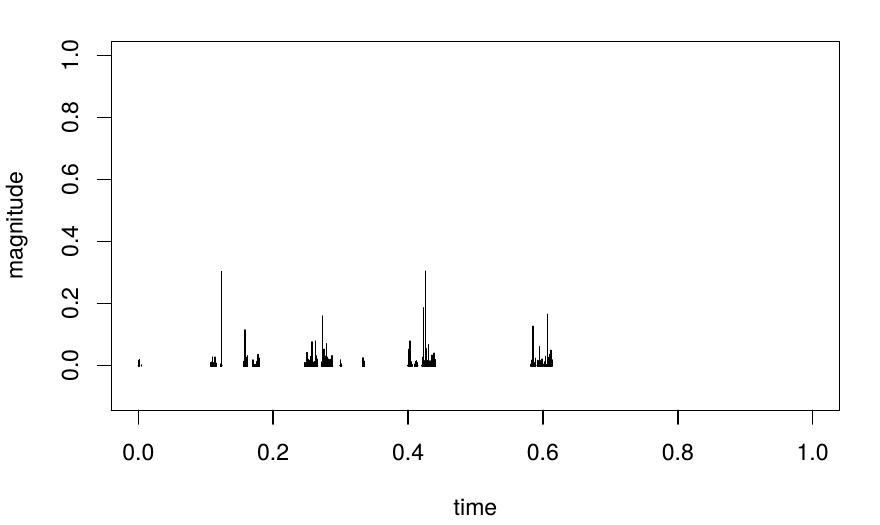
\includegraphics[width=\textwidth]{Figures/unitCTRMprocessNoTitle.png}
        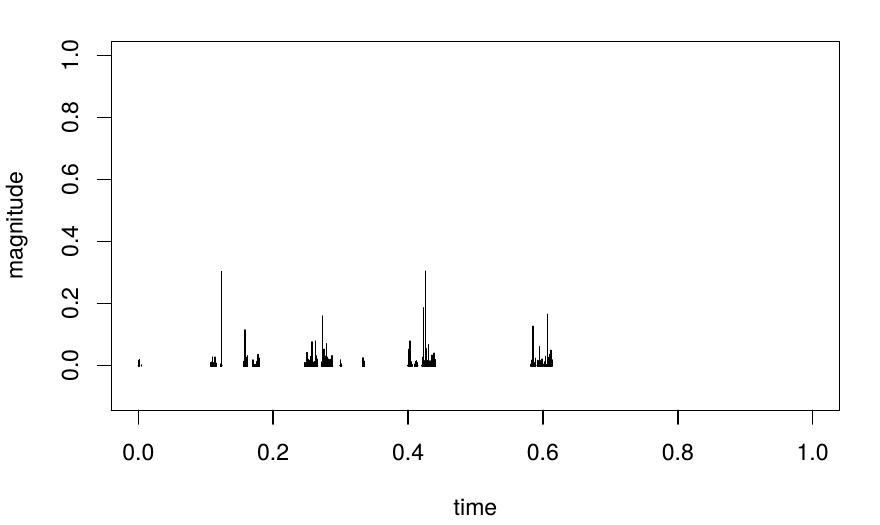
\includegraphics[scale=0.45]{Figures/unitCTRMprocessNoTitle.png}
        %\label{fig:my_label}
    \end{figure}

Recall that we have defined the exceedance duration of level $\ell \in [x_0,x_F]$ as
the random variable
\begin{align*}
T_\ell = \inf\{t: M(t) > \ell\}
\end{align*}
and the exceedance as 
\begin{align*}
X_\ell = M(T_\ell) - \ell.
\end{align*}

As these random variables are the quantities of interest it is natural for us to then consider the (simulated) sample exceedances and their corresponding durations over the threshold level $\ell$.
	
	\begin{figure}[H]
        \centering
        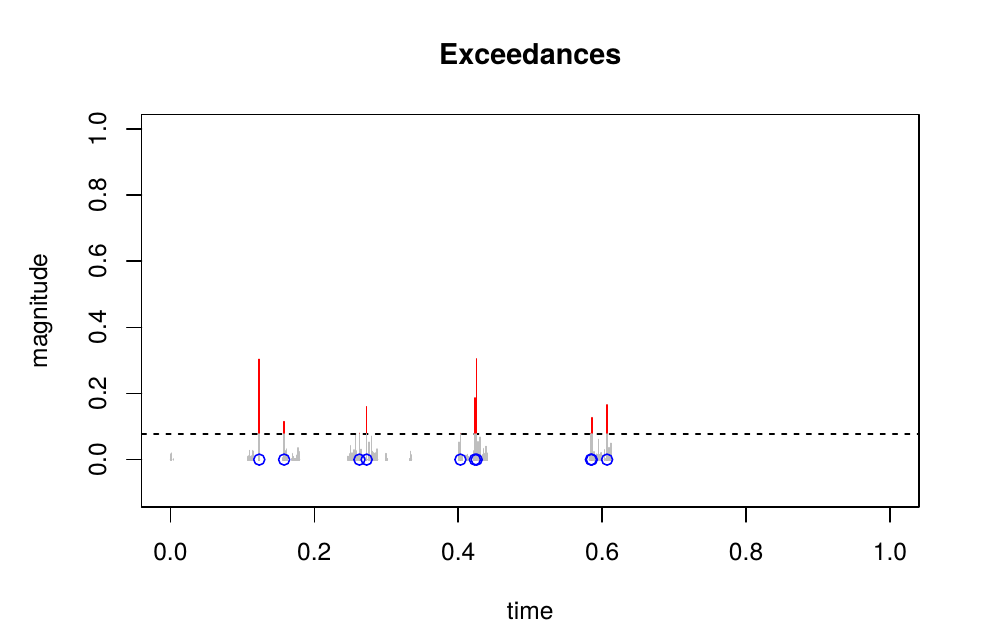
\includegraphics[width=\textwidth]{Figures/Exceedances.png}
        \caption{Exceedance durations (blue circles) and Exceedance sizes (red lines).}
        %\label{fig:my_label}
    \end{figure}


Assume now a time series of magnitudes, and that interest lies in the
estimation of the timings of the large magnitudes.
Consider a minimum threshold $\ell_0$, e.g. at the 95\% quantile.
Vary the threshold $\ell$ on the interval $[\ell_0, x_F]$, and consider
the resulting sequences of exceedance sizes and exceedance times 
$\{(X_{\ell,i}, T_{\ell,i})\}$. 
Due to the renewal property each sequence is i.i.d.. Now $T_{\ell,1}, T_{\ell,2}, \ldots$ can be modelled by a Mittag-Leffler distribution and $J_{\ell,1}, J_{\ell,2}, \ldots$ can be modelled by a Generalised Pareto distribution as shown in chapter \ref{dist}.
\section{Model Fit of Real Data}

\chapter{Conclusion}

%%%%%%%%%%%%%%%%%%%%%%%%%%%%%%%%%%%%%%%%%%%%%%%%%%%%%%%%%%%%%%%%%%%%%%%%%%

\clearpage
\addcontentsline{toc}{chapter}{References}
\bibliographystyle{alpha}
\bibliography{ThesisV1}

\end{document}
